\section{Introduction}\label{sec:introduction}

Knowledge distillation (KD) transfers predictive information from a teacher to a smaller student. Autoregressive LM distillation now includes alternative divergences, on-policy training, adaptive supervision, and teacher selection. These developments make clear that stronger teachers do not automatically produce stronger students. A practical question precedes the choice of a more sophisticated algorithm: given a student that has already been trained, does frozen teacher supervision improve over continuing maximum-likelihood training from exactly the same state?

\begin{figure*}[!t]
\centering
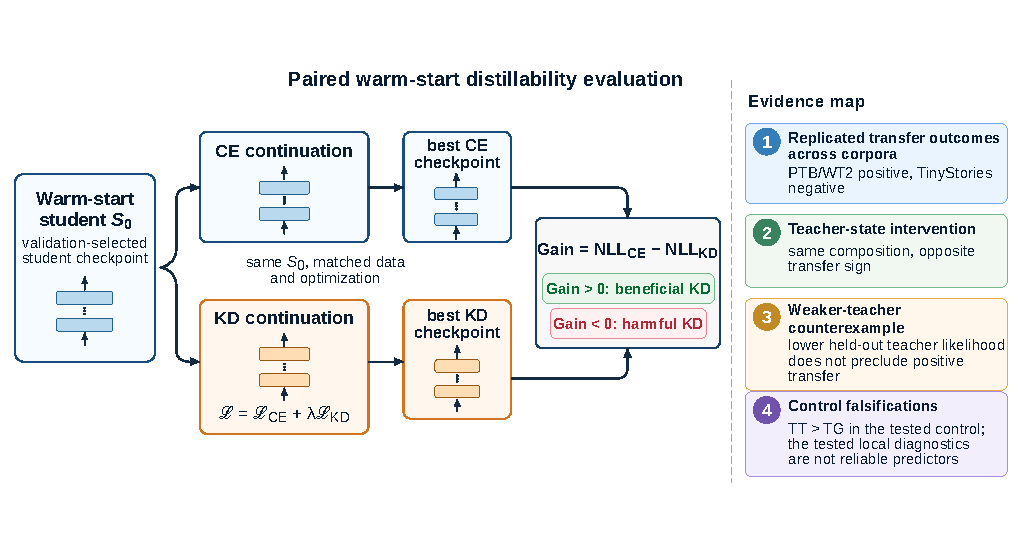
\includegraphics[width=\textwidth]{figures/fig1_paired_protocol.pdf}
\caption{Paired warm-start evaluation. Identical $S_0$ weights initialize CE and KD; independent validation selection precedes test reporting. The evidence map separates replicated transfer from bounded explanatory controls.}
\label{fig:paired_protocol}
\end{figure*}

We study this question through paired warm-start evaluation. A validation-selected student checkpoint $S_0$ initializes both a cross-entropy (CE) continuation and a KD continuation. Both arms use fresh optimizers and matched continuation data and budgets, then independently select checkpoints by validation likelihood. Their test-NLL difference measures the value of adding supervision beyond CE, not improvement over an unrelated baseline. Each confirmatory comparison uses three independently trained student initializations.

This design reveals reproducible positive and negative transfer under the same token-normalized KD formulation. Mean gains are $0.1449$ NLL on PTB and $0.1557$ on WikiText-2, whereas TinyStories degrades by $0.1072$. Every domain has the same direction across all three students. These results do not establish a causal effect of corpus identity: teachers, data amounts, and preparation histories differ. We therefore test candidate explanations with more controlled comparisons.

Teacher quality is an important but incomplete explanation. At fixed WikiText-2 teacher architecture, source identities, and fusion composition, a jointly trained teacher helps all three students, while a fusion-weight-only state harms all three. The paired contrast is $0.1833$ NLL. Teacher training state and resulting predictive quality strongly modulate transfer, but this intervention does not isolate scalar likelihood as the cause. Conversely, a Grassmann-only source with worse held-out likelihood than every matched validation-selected CE comparator still improves all three students. Global teacher likelihood alone therefore cannot determine distillability.

Within a fixed Transformer--Grassmann checkpoint, fused supervision transfers better than either component. A homogeneous Transformer--Transformer control nevertheless yields better KD endpoints in all three students, despite lower branch disagreement. Differences in teacher quality, parameter count, and training history prevent attributing this ordering to architecture. The control does not support uniquely transferable Grassmann representations or heterogeneous-supervision superiority.

Retrospective local gradient and curvature scores also misclassify several configurations with reproducibly positive endpoints. We treat these failures as bounded falsification evidence, not a new predictor or a universal impossibility result. The tested statistics do not summarize the long optimization trajectory and validation selection.

The contribution is a controlled empirical evidence chain: paired CE-relative positive and negative transfer, a fixed-composition teacher-state reversal, a weaker-source counterexample, a homogeneous-ensemble falsification, and failed retrospective local diagnostics. We do not propose a new KD algorithm or claim the first instance of harmful or weak-teacher KD. The practical implication is to assess teacher supervision against matched continuation from the student state of interest, rather than infer its value from a single teacher-quality, diversity, or local-compatibility statistic.
